L'expérience que nous avons réalisé consiste donc à réaliser des transistors moléculaires, afin de caractériser leur comportement.
\section{La réalisation des circuits en salle blanche (faite en amont par Mr Balestro)}
La réalisation des fils d'or a pris plusieurs semaines ; c'est pourquoi Frank Balestro les avait déjà réalisés en salle blanche, au CNRS, avant l'expérience.
Nous avons donc commencé la journée avec 3 plaques de Al$_2$O$_3$, avec chacune 4 groupes de 12 transistors non formés.
\begin{figure}[h]
    \begin{center}
        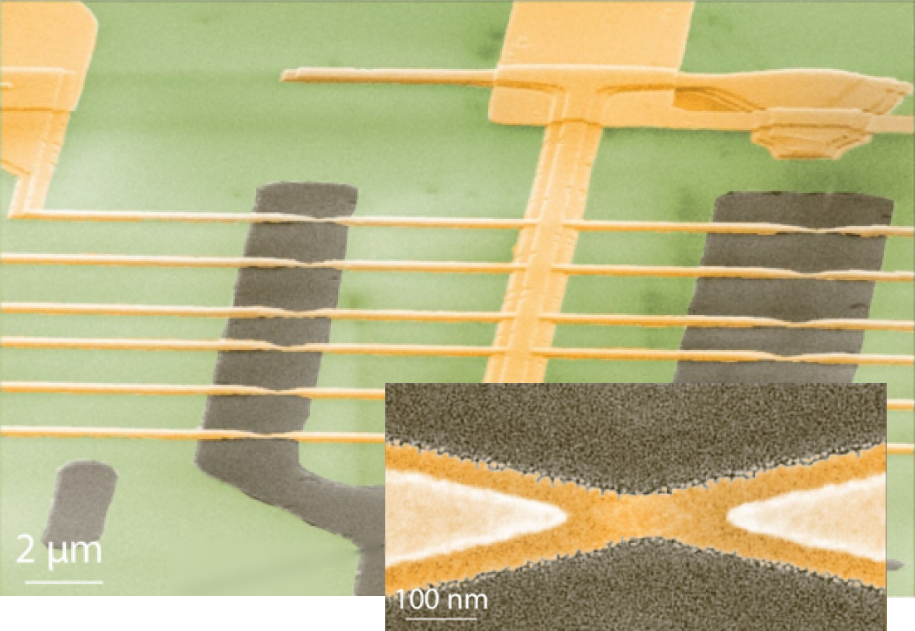
\includegraphics[width=250px]{Images/GroupeDeTransistors}
        \caption{Un groupe de transistors avec grille et source communes}
        \label{fig:}
    \end{center}
\end{figure}
\section{Le dépôt de Fullerène}
Nous sommes donc allés en salle propre de dépôt chimique afin de déposer sur ces plaques le Fullerène, en solution de Toluène.
Cette solution, conservée dans un frigo, est parfaitement inerte, ce qui nous autorise à la conserver très longtemps : celle que nous avons utilisé date de 2009 et est encore utilisable.\\

Le dépôt se fait à l'aide d'une micropipette, et sous hotte aspirante afin d'éviter toute inhalation de fullerène et toute pollution de l'échantillon.
La solution est assez faible en agrégats, et ceux qui ont pu se former se trouvent essentiellement à la surface et au fond de la solution. Nous sommes donc allés récupérer la solution au milieu du bécher.

Le dépôt de fullerène n'a pas besoin d'être mesuré : 3 gouttes de solution par plaque sont suffisantes pour obtenir une probabilité acceptable qu'une molécule se glisse dans le nanogap après électromigration.

Enfin, nous avons laissé s'évaporer le Toluène naturellement.
\section{Une expérience à 4.2K grâce à l'hélium liquide}
Une fois le Fullerène déposé, nous avons fixé les plaques sur un plateau. La fixation se fait à la laque d'argent.

Dans le testeur sous pointes, l'échantillon sera dans une cavité sous vide (vide secondaire de l'ordre de 4-10 millibars). L'unique contact thermique avec les échantillons sera donc par ce plateau. Celui-ci doit être efficace. Sinon, les échantillons seront à haute température et nous n'aurons donc pas du tout le comportement attendu.

L'argent est un très bon conducteur thermique et la laque d'argent permet d'avoir un contact uniforme entre les échantillons et le plateau.

De plus, l'argent nous permet d'avoir une bonne mise à la masse des échantillons et donc de minimiser les risques de choc électrique qui risqueraient de détruire les jonctions formées.
\begin{figure}[h]
    \begin{center}
        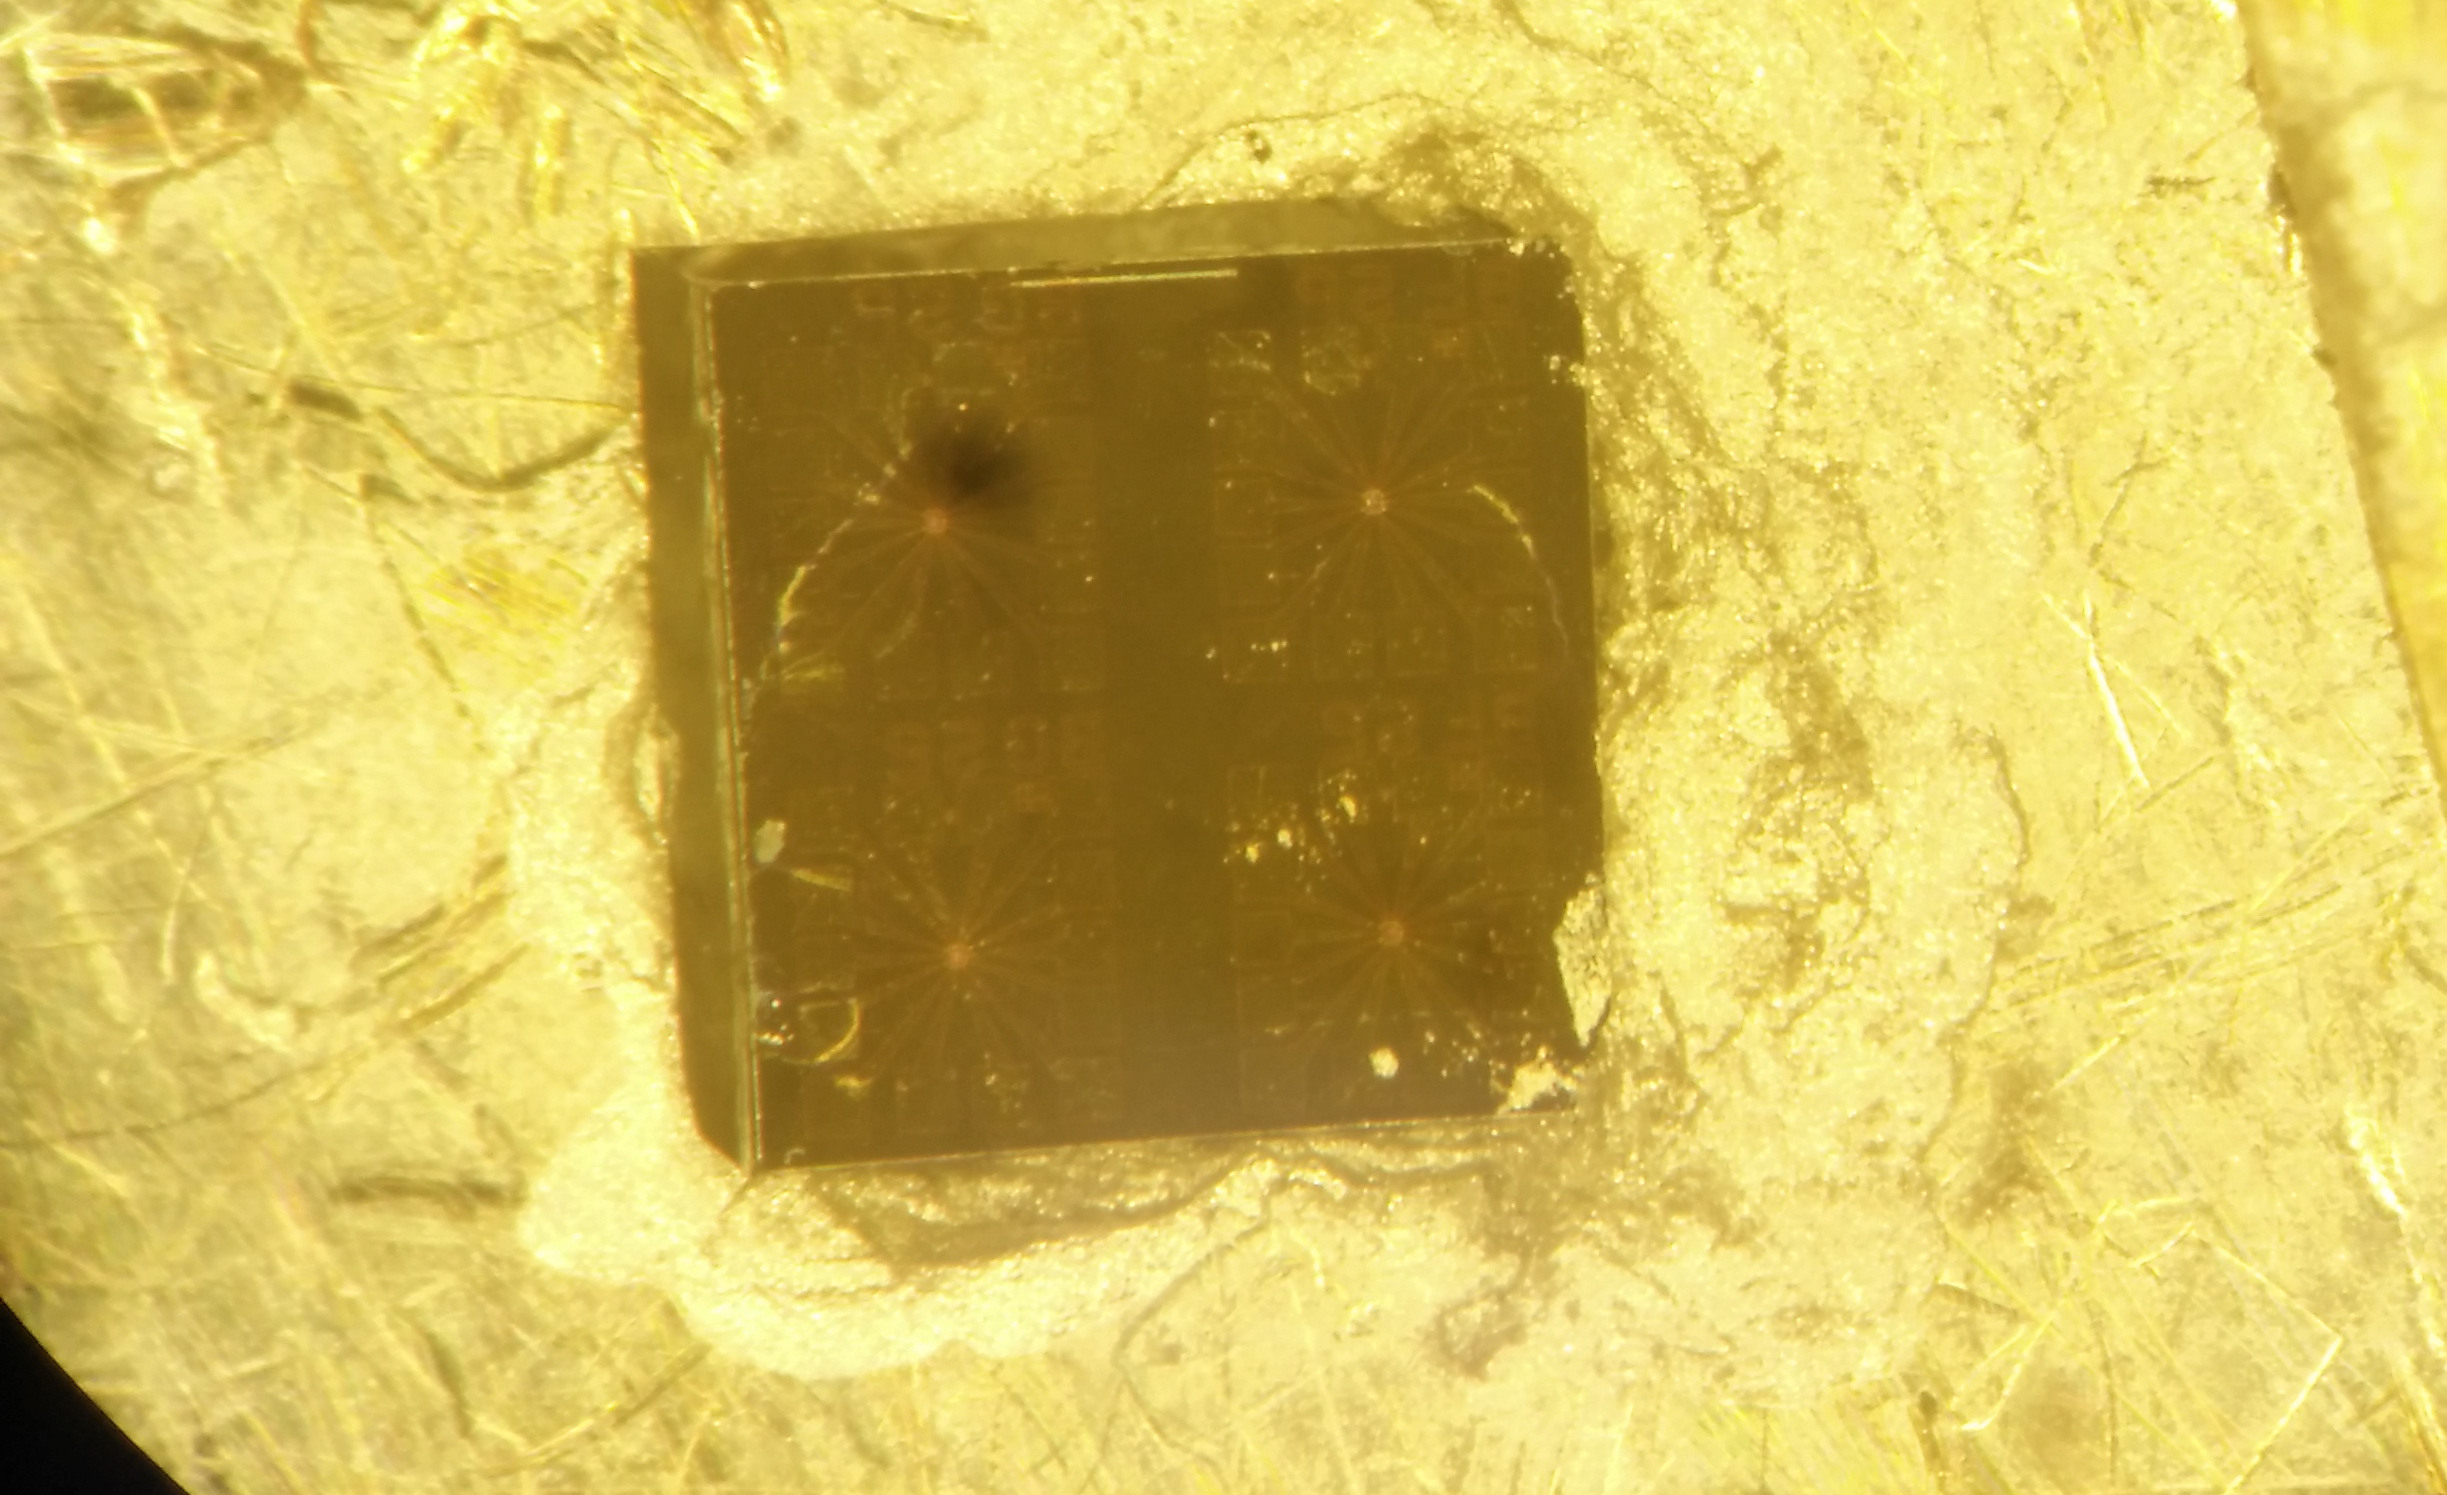
\includegraphics[width=250px]{Images/PhotoPlaqueTransistors}
        \caption{Échantillon collé à l'aide de laque d'argent}
        \label{fig:}
    \end{center}
\end{figure}

Pour empêcher un maximum le réchauffement du au rayonnement l'échantillon est placé sous deux écrans. Le premier  écran est à 10K est placé au niveau du hublot. Le deuxième écran est à 300K (température de la pièce). On peut alors efficacement refroidir à 4.2K. Au préalable, il a fallu faire le vide entre les deux écrans et l'écran intermédiaire et l'échantillon pour empêcher tout réchauffement par conduction ou convection et  pour empêcher que l'air ne gèle autour de l'échantillon ce qui interdirait toute manipulation.
\subsection{L'Hélium Liquide}
Comme dit précédemment, nous pouvons effectuer cette expérience à 4.2K grâce à l'Hélium liquide. Et, heureusement, l'hélium liquide est facile d'accès à l'Institut Néel.

Il nous faut donc transporter la bouteille d'hélium liquide vide jusqu'au centre de liquéfaction, pour prendre une bouteille pleine. Il faut aussi indiquer les poids des bouteilles entrante et sortante, afin d'attribuer la consommation à tel ou tel laboratoire.

La manipulation de la bouteille d'hélium doit se faire avec précaution. En effet, le haut de la bouteille est “chaud”, donc en cas de contact brusque avec l'hélium liquide, celui-ci se dilate très rapidement, ce qui transforme la bouteille d'hélium en “torpille”.
\begin{figure}[h]
    \begin{center}
        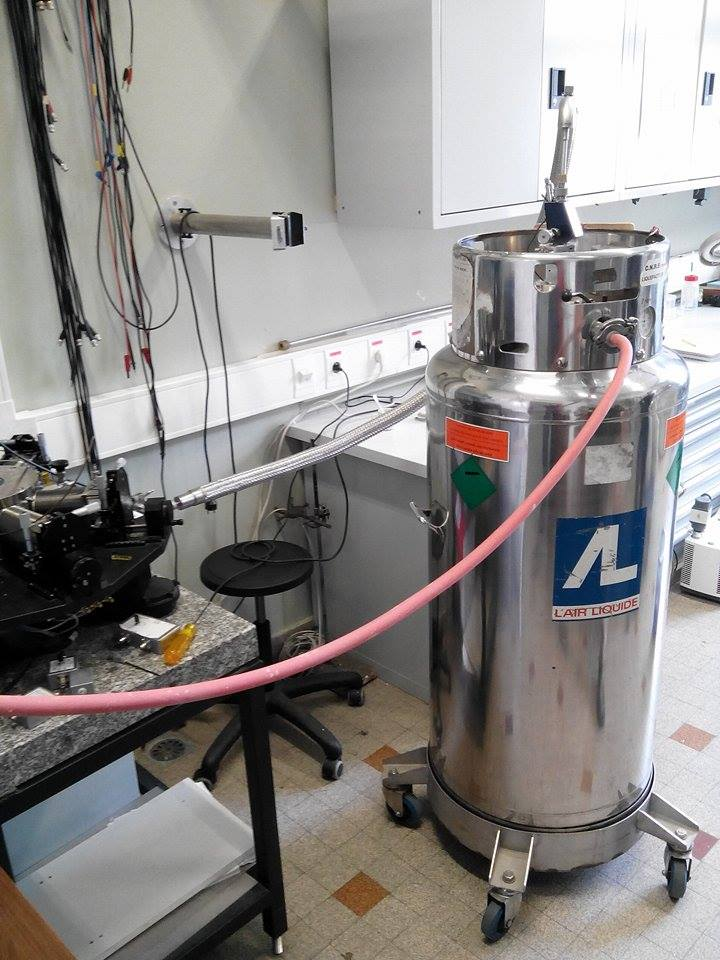
\includegraphics[width=150px]{Photos/Bouteille_Helium_Liquide.jpg}
        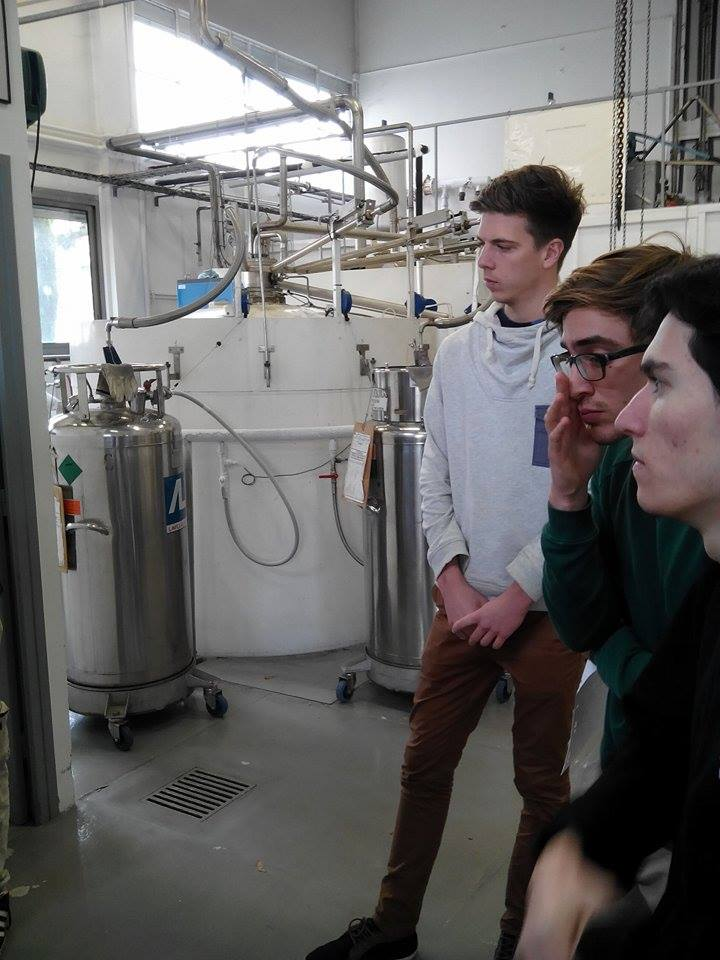
\includegraphics[width=150px]{Photos/Centre_Helium_Liquide.jpg}
        \caption{Une bouteille d'Hélium Liquide et le centre de liquéfaction.}
        \label{fig:}
    \end{center}
\end{figure}

\section{Les méthodes de mesure}
\subsection{La mesure de résistivité}
Afin de vérifier que nos pointes sont bien connectées et qu'il y a bien un nanofil entre elles, on utilise un ohmmètre spécialisé délivrant des micro-ampères. En effet la largeur de transport est de quelques atomes d'or et un courant classique de l'ordre du mA détruirait immédiatement nos échantillons.
Nous polarisons nos échantillons en tension, et cherchons donc à mesurer le courant traversant les échantillons.
On transforme le courant en une tension par l'intermédiaire d'un convertisseur courant-tension présentant différents facteurs, afin d'effectuer nos mesures. Lors de l'électromigration on utilise un facteur $10^3$ pour mesurer des uA.
Pour observer les diamants de Coulomb on mesure des faibles courant (nA),  on sélectionne le facteur $10^6$ sur le convertisseur. 

\begin{figure}[h]
    \begin{center}
        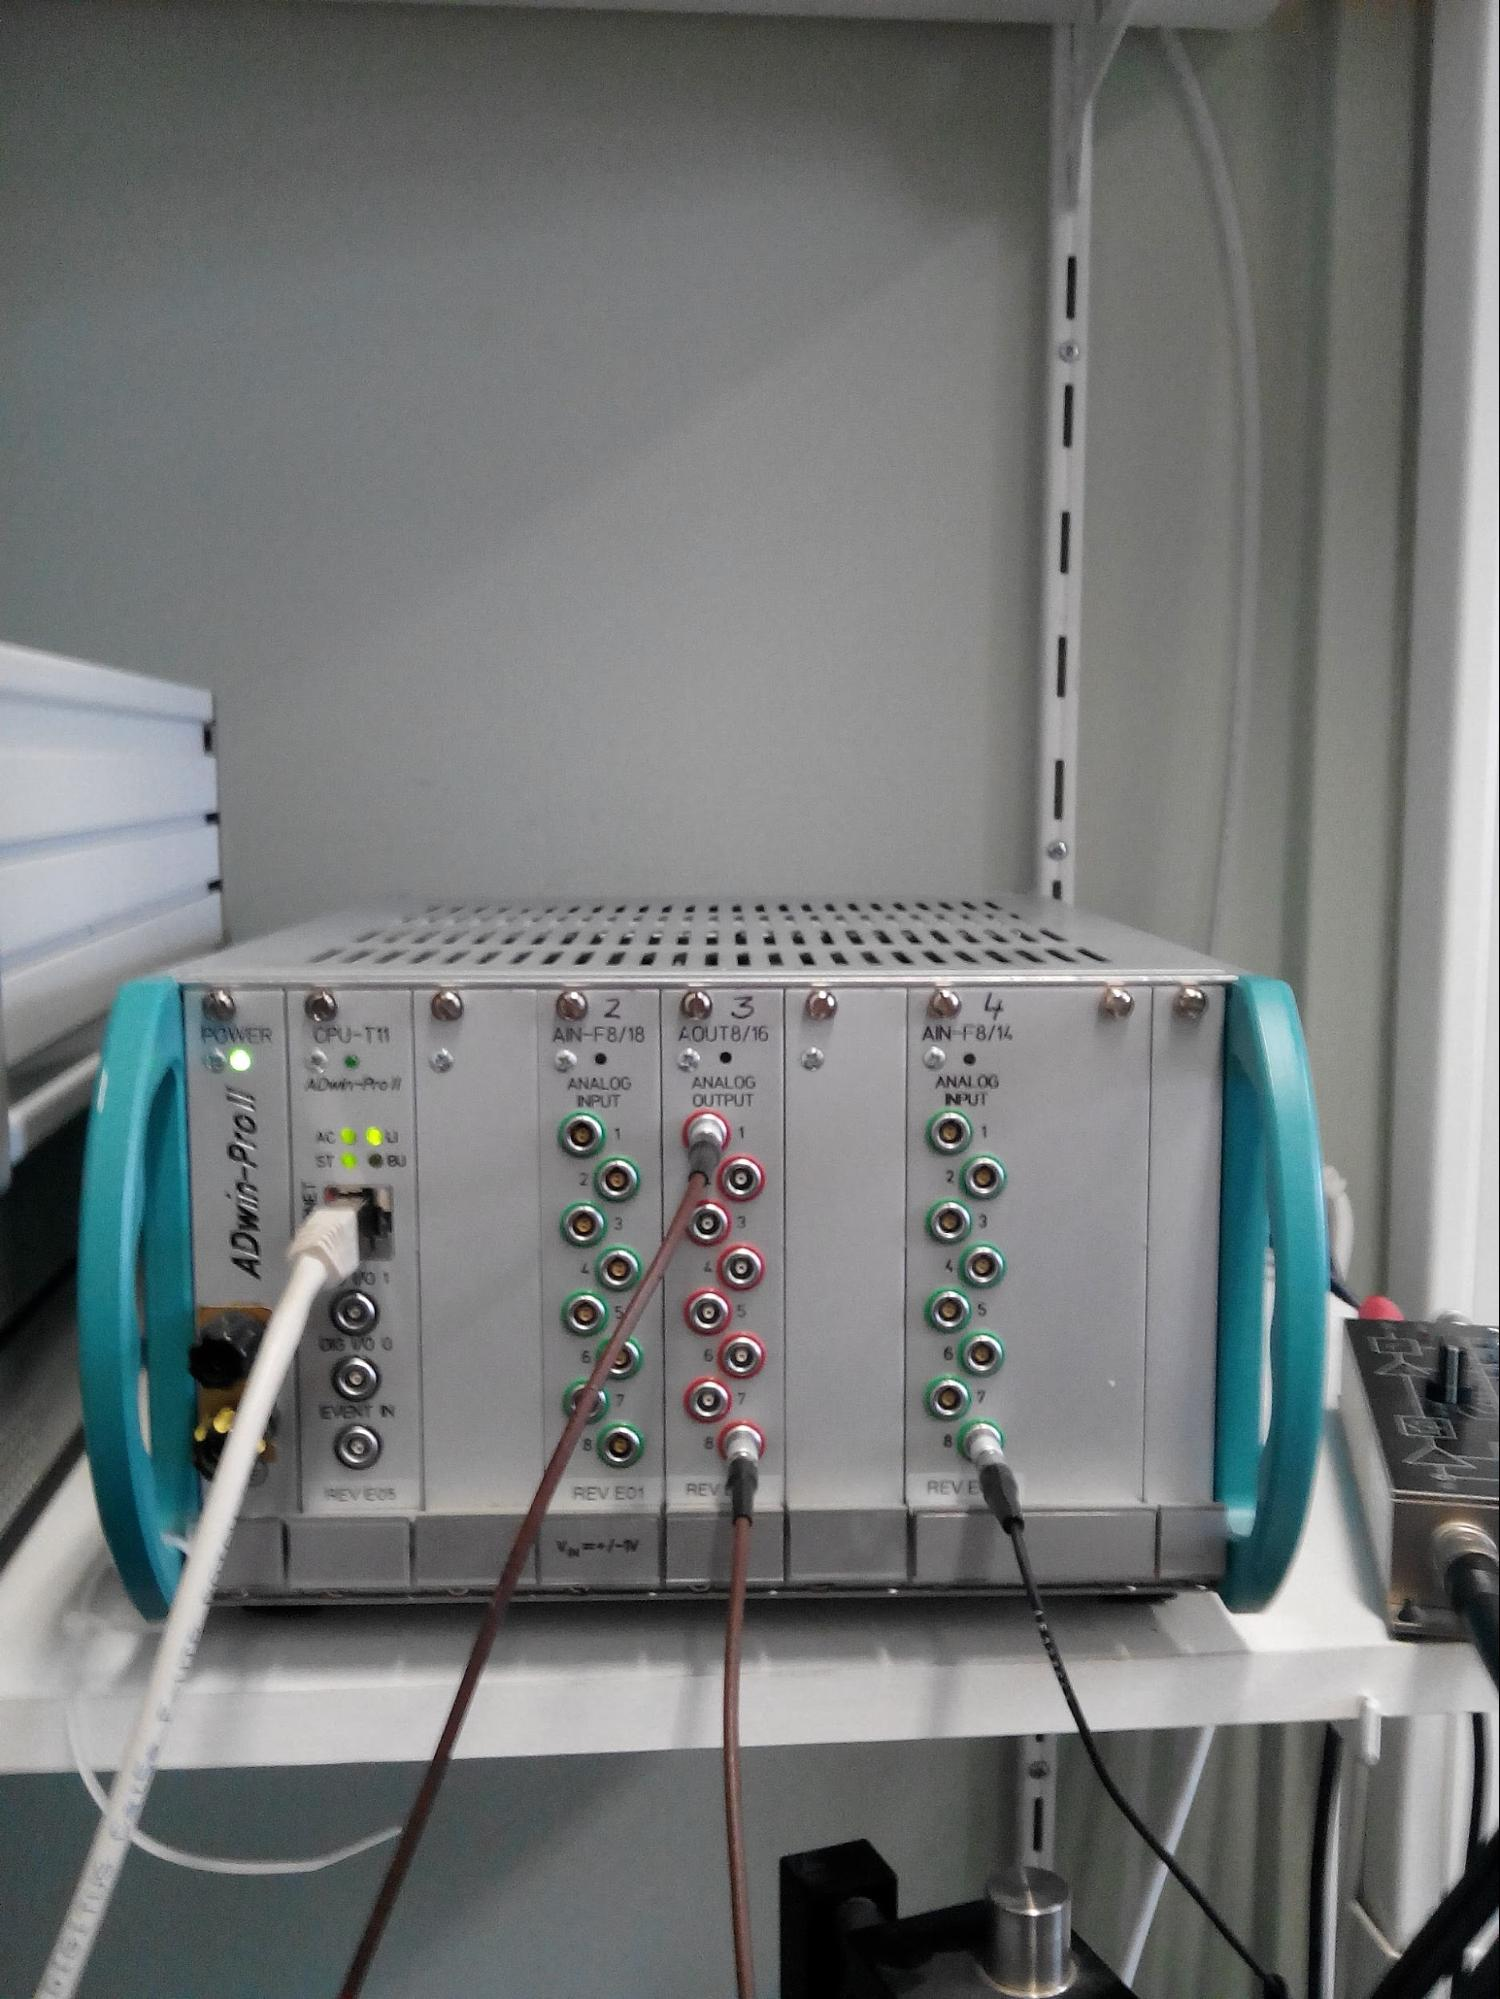
\includegraphics[trim=0mm 0mm 80px 600px, clip, width=200px]{Photos/Branchements_ADWin.jpg}
        \caption{Branchements de l'interface Adwin lors de l'électromigration, on peut voir sur la droite le convertisseur courant-tension}
        \label{fig:}
    \end{center}
\end{figure}


\subsection{Les précautions à prendre}
Lorsqu'on manipule de tels échantillons, il faut bien sûr prendre quelques précautions afin de ne pas les détériorer définitivement.
Dans le testeur sous pointes, les échantillons sont à l'abri des perturbations extérieures : la structure de l'appareil, et particulièrement le plateau sur lequel les échantillons sont posés, sont mis à la masse.
Le principal risque vient donc des pointes : Si on les fait bouger alors qu'une tension est appliquée, le risque de pics de tension est très élevé. Avant chaque mesure et déplacement des pointes, nous faisons donc attention à les mettre à la masse. Cela peut être répétitif, mais absolument indispensable. 

\section{L'électromigration}
L'électromigration consiste, comme nous l'avons expliqué précédemment, à appliquer à l'échantillon une tension suffisamment forte pour “détruire” le fil d'or et créer un nanogap.
ADWin nous permet d'avoir une mesure suffisamment rapide du courant et d'arrêter l'électromigration suffisamment rapidement pour ne pas risquer d'abîmer le nanogap créé.
Nous pouvions observer en temps réel les courbes de courant et de résistivité de l'échantillon. Pour un échantillon correct nous observions bien la rampe de tension appliquée puis le comportement classique d'électromigration, dont la chute par paliers du courant.
Pour un échantillon abîmé -- ce fut malheureusement le cas pour beaucoup, dû à un problème en salle blanche en amont --, nous pouvions observer une résistivité qui croit linéairement dès l'application de la tension.
\section{L'étude du blocage de Coulomb}
Après avoir effectué l'électromigration avec succès sur un échantillon, il nous fallait vérifier la présence d'une molécule de Fullerène dans le nanogap tout juste créé.  Pour cela, on mesure le courant Id en faisant varier la tension appliqué à la grille. Si aucun courant n'est observé, alors aucune molécule de Fullerène ne s'est logée à l'intérieur du nanogap. Si l'on observe des pics de courant pour certaines valeurs discrètes de Vg, c'est que l'on est en présence d'une boite quantique. Lorsque les conditions sont vérifiées par rapport aux équations établies dans la partie théorique, le courant peut passer ou non. On contrôle donc un courant  à partir d'une tension appliquée à une électrode de grille : on vient donc de réaliser un transistor à molécule unique.

On peut aussi observer le courant pour des valeurs variables de Vg et Vds. Le courant Id mesuré est représenté en 3ème dimension ou en couleurs. Nous pouvons alors observer la forme caractéristique des diamants de Coulomb, dont la frontière correspond aux pics de courant évoqués précédemment.
